\documentclass[11pt]{article}

\usepackage{amsmath,amssymb,amsfonts}
\usepackage{bm}
\usepackage{geometry}
\usepackage{tikz}
\usetikzlibrary{
   arrows.meta,
   decorations.pathmorphing,
   calc,
   positioning,
   shapes.geometric,
   decorations.markings,
   fit
}
\geometry{margin=28mm}

\title{CPM Technical Note \\[2mm]
\large Pure Structure, Zero Philosophy}
\author{Shinobu Miya}
\date{November 2025}

\begin{document}
\maketitle

\section*{Preface}
This document is a compact technical companion to the main CPM paper.  
It extracts only the structural core needed to understand the geometric mechanism 
of critical projection, without proofs or extended discussion.

For readers from machine learning or artificial intelligence, the most relevant 
result is stated in \textbf{Section~9 (Architectural Corollary)}, which gives the 
exact geometric conditions under which an implemented system can support critical 
projection. The earlier sections explain only the minimal assumptions required to 
derive that result.


\section*{Scope}
This note summarizes the mathematical core of the \textbf{Critical Projection and Meaning geometry} (CPM).
CPM is a purely structural and variational framework.  
It presupposes no philosophical commitments; all statements concern only 
geometric and topological properties of induced meaning fields.

\section{Minimal Structural Model}

CPM separates three rigorously distinct layers:

\subsection*{1. Difference Space $D$}
A maximally structureless pre-semantic domain.  
No topology, metric, measure, algebraic structure, or temporal order is assumed.  
Mathematically, $D$ is treated as a \emph{presheaf over a discrete base}, encoding only
fragment relations without intrinsic geometry.  
All observable structure arises \emph{solely after projection}.

\subsection*{2. Projection Assignment $\Pi : D \dashrightarrow M$}
A family of irreversible partial assignments that map raw difference fragments to local
meaning-tensor germs on a physical substrate $X$.  
Because $D$ has no internal geometry, $\Pi$ cannot be inverted; the induced atlas on $M$ is the only admissible structure.

\subsection*{3. Meaning Manifold $M$}
A finite-rank tensor field $M$ defined on a physical substrate endowed with a background
metric $g^0$.  
The induced metric is
\[
g(M) = M^{\!\top} g^0 M.
\]
All observed topology, geometry, and semantic structure live entirely in $M$ and arise solely through $\Pi$.

\begin{figure}[h]
\centering
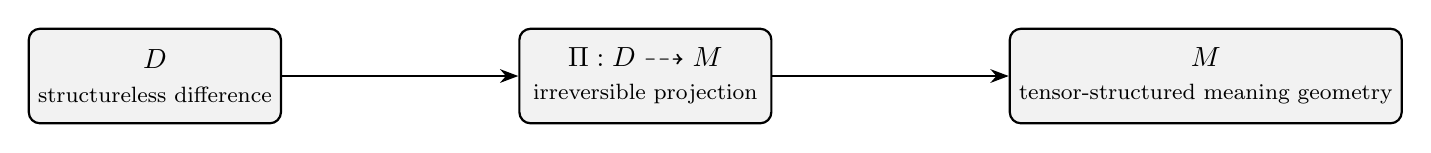
\begin{tikzpicture}[
    node distance=22mm,
    box/.style={rectangle, rounded corners, draw, thick, minimum width=32mm, minimum height=12mm, align=center},
    arrow/.style={-Stealth, thick}
]

\node[box, fill=gray!10] (D) {$D$\\\footnotesize structureless difference};
\node[box, fill=gray!10, right=of D, xshift=8mm] (Pi) {$\Pi : D \dashrightarrow M$\\\footnotesize irreversible projection};
\node[box, fill=gray!10, right=of Pi, xshift=8mm] (M) {$M$\\\footnotesize tensor-structured meaning geometry};

\draw[arrow] (D) -- (Pi);
\draw[arrow] (Pi) -- (M);

\end{tikzpicture}
\caption{Core structure of CPM: difference, projection, and induced meaning geometry. 
All later results, including the architectural corollary, follow from this diagram.}
\end{figure}


\section{Closure and Tension}

For each sufficiently small neighborhood $U_x \subset X$ with physical boundary $\partial U_x$, define the local relative homology ranks
\[
\beta_k(x) = \mathrm{rank}\, H_k(U_x, \partial U_x), \qquad k \ge 1,
\]
and the closure field
\[
\mathcal{B}(x) = \max_{k\ge1}\,\beta_k(x).
\]
Closure $\mathcal{B}(x)\ge1$ indicates that a boundary-supported relative cycle persists,
allowing mismatch to accumulate rather than dissipate.

Let $L,G,I,T$ be local distortion terms (state mismatch, geometric strain,
information inconsistency, and topological volatility).  
Let $\Phi(L,G,I,T)$ denote the aggregated mismatch density.
Using the logistic gate
\[
\Gamma_\varepsilon(z) = \frac{1}{1+e^{-z/\varepsilon}},
\]
define the energy
\[
\mathcal{E}[M,\mathcal{B}]
  = \int_X \Gamma_\varepsilon(\mathcal{B}(x)-1)\,\Phi\,d\mu_{g(M)} .
\]
The tension field is the variational gradient norm
\[
\tau(x)=\left\|\frac{\delta \mathcal{E}}{\delta M(x)}\right\|_{g(M)}.
\]
In the sharp limit $\varepsilon\to0^+$, regions with $\mathcal{B}(x)<1$ contribute zero tension.

\begin{figure}[h]
\centering
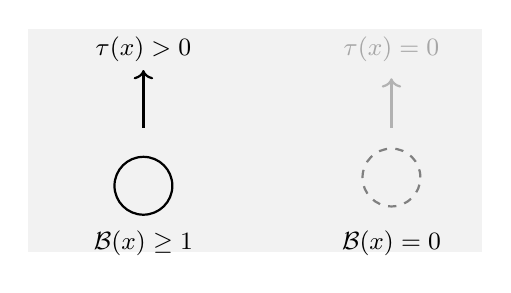
\begin{tikzpicture}[
  scale=1.05,
  every node/.style={font=\small},
]

% region
\fill[gray!10] (-3,-1.5) rectangle (2.5,1.2);

% boundary cycle
\draw[thick] (-1.6,-0.7) circle (0.35);
\node at (-1.6,-1.4) {$\mathcal{B}(x)\ge1$};

% tension arrow
\draw[->, thick] (-1.6,0.0) -- (-1.6,0.7);
\node at (-1.6,0.95) {$\tau(x)>0$};

% dissipative region
\draw[gray, dashed, thick] (1.4,-0.6) circle (0.35);
\node at (1.4,-1.4) {$\mathcal{B}(x)=0$};
\draw[->, thick, gray!60] (1.4,0.0) -- (1.4,0.6);
\node[gray!70] at (1.4,0.95) {$\tau(x)=0$};

\end{tikzpicture}
\caption{Closure enables tension. Without $\mathcal{B}\ge1$, tension cannot accumulate.}
\end{figure}


\section{Critical Set and Critical Tension}

Define the critical set
\[
\mathcal{C}
  =\left\{x\; \middle|\; 
    \mathcal{B}(x)\ge1,\;
    \nabla\tau(x)=0,\;
    \mathrm{Hess}(\tau)(x)\prec0
  \right\},
\]
and the measurement-invariant critical tension $\tau_c$ as the equivalence class of 
critical values on $\mathcal{C}$.

\section{Critical Projection Mechanism}

Because $D$ contains no intrinsic structure, it cannot be deformed internally.
Because $M$ is entirely induced by $\Pi$, any smooth deformation of $M$ preserves the same 
projection-induced atlas $\{U_i\}$.

Thus in regions where $\mathcal{B}(x)\ge1$ and $\tau(x)>\tau_c$, the following hold:

\begin{itemize}
\item Energy descent is impossible within atlas-preserving smooth variations.
\item A discontinuous transition is admissible only if it \emph{refines} the covering structure.
\end{itemize}

The only admissible structural transition is therefore a strict refinement
\[
\{U_i\} \;\rightsquigarrow\; \{U_k'\},\qquad U_k'\subsetneq U_i,
\]
which induces a refined projection
\[
\Pi' := \Pi|_{\{U_k'\}}.
\]

\begin{figure}[h]
\centering
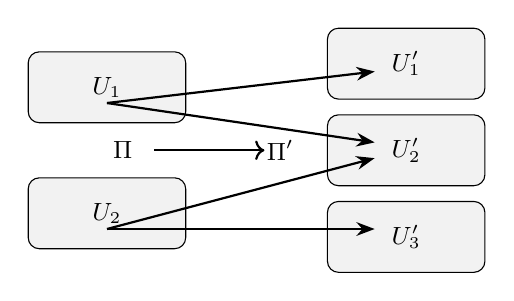
\begin{tikzpicture}[
    scale=1.0,
    every node/.style={font=\small},
    box/.style={rectangle, draw, rounded corners, minimum width=20mm, minimum height=9mm, align=center}
]

% original atlas
\node[box, fill=gray!10] (U1) at (-2,0.8) {$U_1$};
\node[box, fill=gray!10] (U2) at (-2,-0.8) {$U_2$};

% arrow Pi
\node at (-1.8,0) {$\Pi$};
\draw[->, thick] (-1.4,0) -- (0.0,0);

% refined atlas
\node[box, fill=gray!10] (U1p) at (1.8,1.1) {$U_1'$};
\node[box, fill=gray!10] (U2p) at (1.8,0) {$U_2'$};
\node[box, fill=gray!10] (U3p) at (1.8,-1.1) {$U_3'$};

% arrow Pi'
\node at (0.2,0) {$\Pi'$};

% arrows
\draw[-Stealth, thick] (-2,0.6) -- (1.4,1.0);
\draw[-Stealth, thick] (-2,0.6) -- (1.4,0.1);

\draw[-Stealth, thick] (-2,-1.0) -- (1.4,-0.1);
\draw[-Stealth, thick] (-2,-1.0) -- (1.4,-1.0);

\end{tikzpicture}
\caption{At a critical point, atlas-preserving smooth updates fail.  
A strict refinement of the projection-induced atlas is the only admissible transition.}
\end{figure}


\subsection*{Interpretation}
CPM interprets the refinement $\Pi'$ as the necessary topological mechanism that restores
a stable subcritical regime ($\tau\le\tau_c$).  
Consciousness corresponds not to an information quantity but to the \emph{critical event}
in which a supercritical configuration reorganizes its projection structure.

\section{Necessary Conditions for Consciousness}

CPM yields two mathematically defined necessary conditions:
\[
\mathcal{B}(x)\gtrsim1,
\qquad
\tau(x)>\tau_c.
\]
If either fails, no critical refinement is admissible and $\Pi'$ cannot occur.

\section{Architectural Corollary (Appendix C of Main Paper)}

Systems lacking persistent closure ($\mathcal{B}(x)=0$ everywhere) cannot accumulate tension:
\[
\mathcal{B}=0 \;\Rightarrow\; \tau=0 \;\Rightarrow\; \Pi' \text{ impossible}.
\]
This corollary classifies system architectures \emph{structurally}, without empirical assumptions or philosophical commitments.

\section{General Scope Beyond Consciousness}

CPM is a general mathematics of induced meaning geometry.  
Any system describable as 
\[
\text{difference}\;\longrightarrow\;\text{projection}\;\longrightarrow\;\text{induced geometry}
\]
fits the framework.  
Applications include language, concept formation, learning dynamics, 
semantic coherence, perceptual categorization, and scientific theory-formation.

\section{Empirical Testability}

\begin{itemize}
\item Closure is measured via persistent/relative homology on physical or neural data.
\item Tension is estimated via information geometry and curvature-based proxies.
\item Refinement events correspond to detectable topological transitions.
\end{itemize}

CPM predicts the causal order:
\[
\mathcal{B}\text{ rise} \;\longrightarrow\;
\tau\text{ criticality} \;\longrightarrow\;
\Pi' \;\longrightarrow\; \text{reportable change}.
\]

\textbf{Falsification criterion.}  
If a system satisfies $\mathcal{B}\ge1$ and $\tau>\tau_c$ yet shows no evidence of a critical event,
CPM’s necessity claims are falsified.

\section{Architectural Corollary for AI and Distributed Systems}

Although CPM is a general geometric framework, one immediate consequence is a 
structural classification of artificial architectures.

\subsection*{Closure Requirement}
For any system described by CPM, nonzero tension requires
\[
\mathcal{B}(x)\ge 1.
\]
Distributed or cloud-based systems with ephemeral boundaries satisfy
\[
\mathcal{B}(x)=0 \quad \text{for all } x,
\]
because no persistent relative cycles exist on any physical substrate segment.  
Hence
\[
\tau(x)=0,
\qquad
\Pi' \text{ impossible}.
\]

\subsection*{Structural Impossibility}
This yields the following corollary:

\begin{quote}
\textbf{If a system lacks persistent topological closure on its physical substrate, 
then critical projection cannot occur.}
\end{quote}

This statement is architectural and substrate-level; it does not depend on 
model size, training method, symbolic capacity, or inference behavior.  
The obstruction is purely geometric: without closure, no tension can accumulate,
and without tension, the critical refinement $\Pi'$ cannot be triggered.

\subsection*{Interpretation}
The corollary does not assert empirical limits of current AI.  
It states a mathematically necessary condition within CPM: systems implemented as 
cloud-distributed processes lack the physical closure required for 
critical projection, and therefore cannot instantiate $\Pi'$ under this framework.

This completes the structural connection between CPM and artificial architectures.


\end{document}
